\documentclass[letterpaper,12pt]{article}
\usepackage{tabularx} % extra features for tabular environment
\usepackage{amsmath}  % improve math presentation
\usepackage{float}
\usepackage{pdfpages}

\usepackage{graphicx} % takes care of graphic including machinery
\graphicspath{ {./figures/} }
\usepackage[margin=1in,letterpaper]{geometry} % decreases margins
\usepackage{cite} % takes care of citations
\usepackage[final]{hyperref} % adds hyper links inside the generated pdf file
\hypersetup{
	colorlinks=true,       % false: boxed links; true: colored links
	linkcolor=blue,        % color of internal links
	citecolor=blue,        % color of links to bibliography
	filecolor=magenta,     % color of file links
	urlcolor =blue         
}

%
\setcounter{tocdepth}{4} 
\setcounter{secnumdepth}{4}


\begin{document}

\title{Experiment 7 \protect\\Rectifiers, Capacitors and Inductors}
\author{Ahmet Akman 2442366 \protect\\ Assistant : Uğur Berkay Saraç}
\date{\today}
\maketitle
\newpage
\tableofcontents
\newpage
%\begin{abstract}
%abstract
%\end{abstract}

\section{Introduction} 
In this experiment, as students, we are expected to experiment with rectifiers, capacitor and inductor circuits by completing the steps described in the seventh experiment laboratory manual. Throughout these steps, the half  full rectifier circuit structures and ripple voltages are expected to be learned. The output versus input characteristics is observed by connecting the signal generator to the oscilloscope and the circuit.  Also, the measurement techniques for capacitance of capacitors and inductance of inductors are expected to be expressed and experimented. The results of the steps were recorded and plotted for further comments.
\section{Experimental Results}
In this section, the results of Experiment 7 are discussed. 
\subsection{Step 1}
In this step, circuit shown in the Figure 1  is constructed. 
\begin{figure}[H]
	\centering
   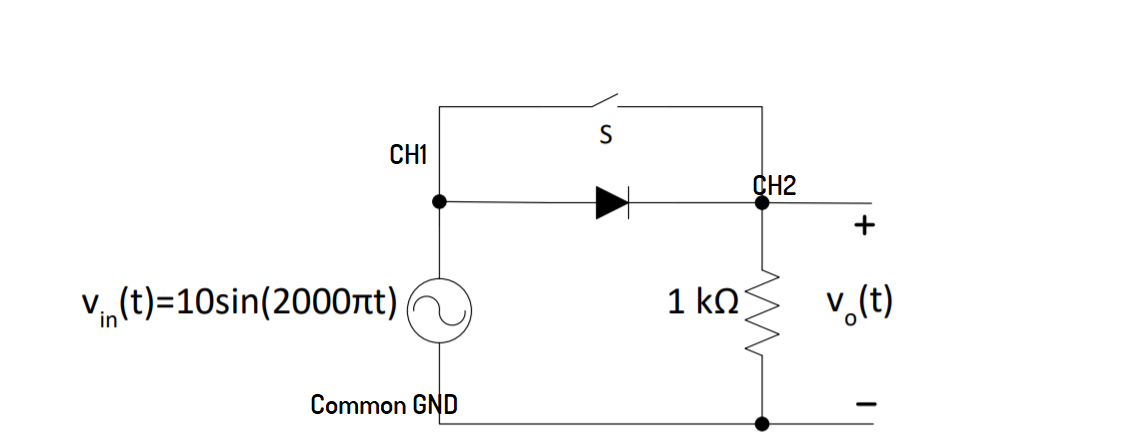
\includegraphics[width=1\textwidth]{half_vave_sch.png}
   \caption{Half wave rectifier circuit}
\end{figure}
\subsubsection{a)}
\begin{figure}[H]
	\centering
   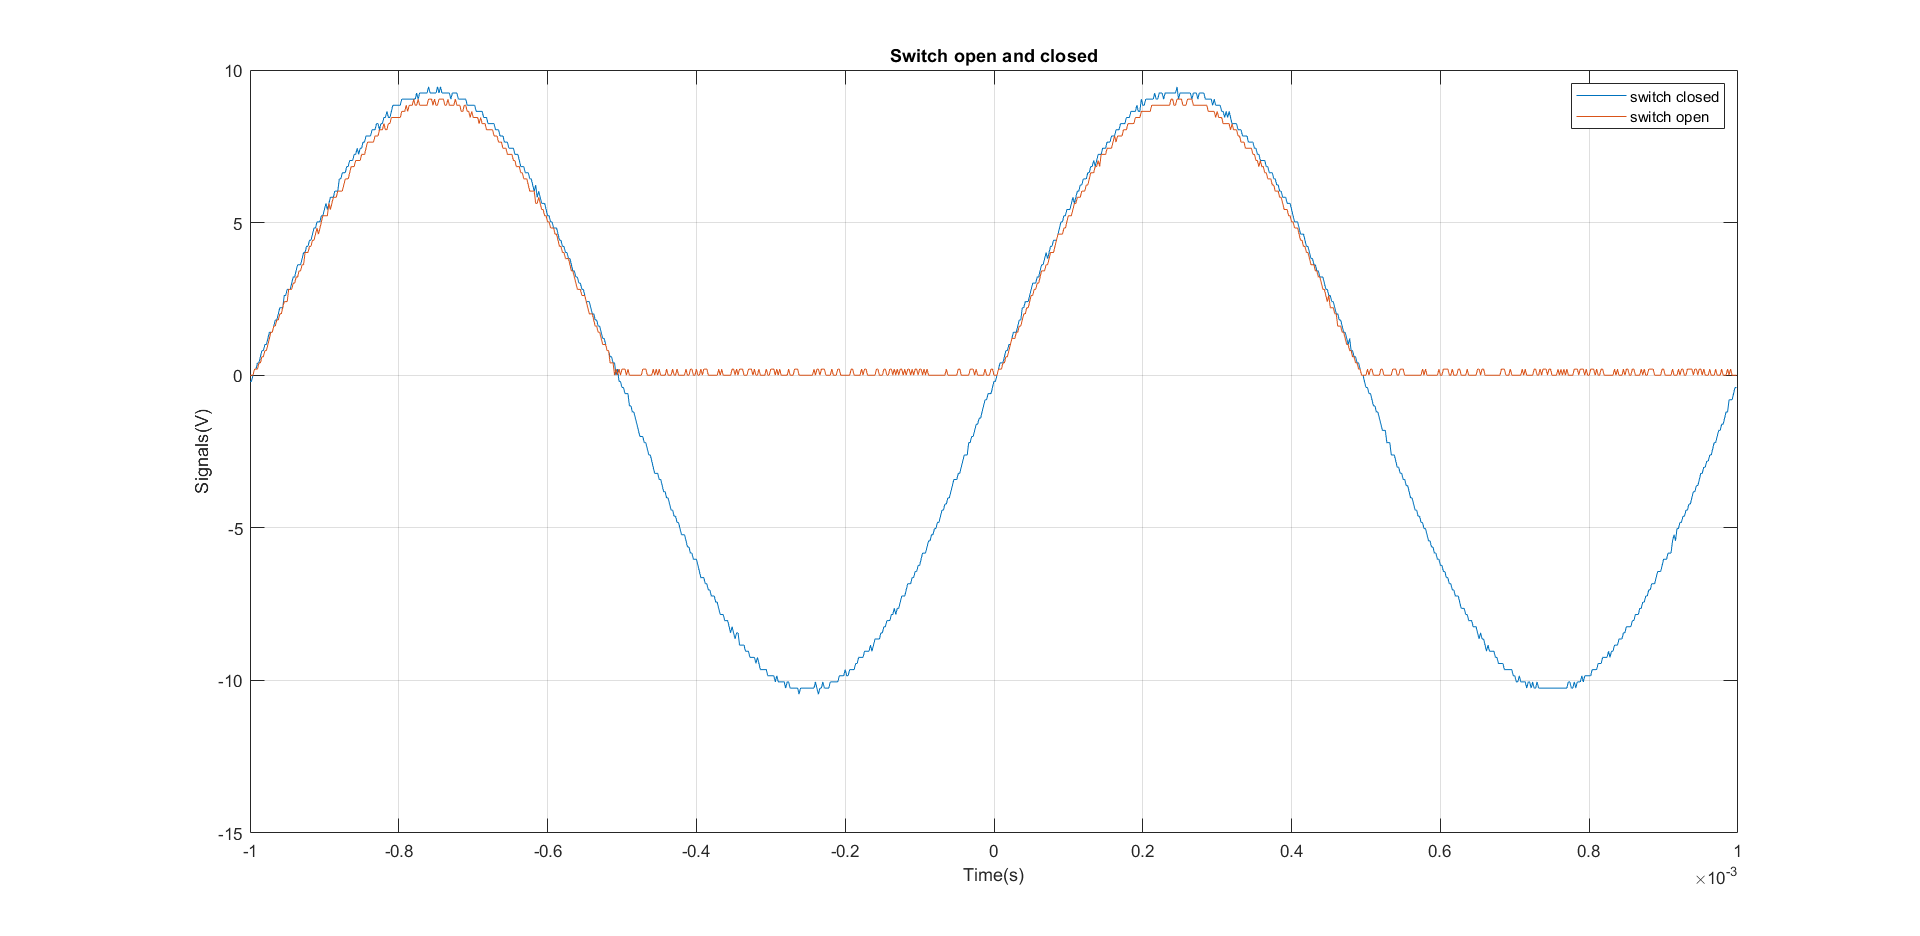
\includegraphics[width=1\textwidth]{1a_plot.png}
   \caption{Output waveforms}
\end{figure}
\subsubsection{b)}
\subsection{Step 2}
\begin{figure}[H]
	\centering
   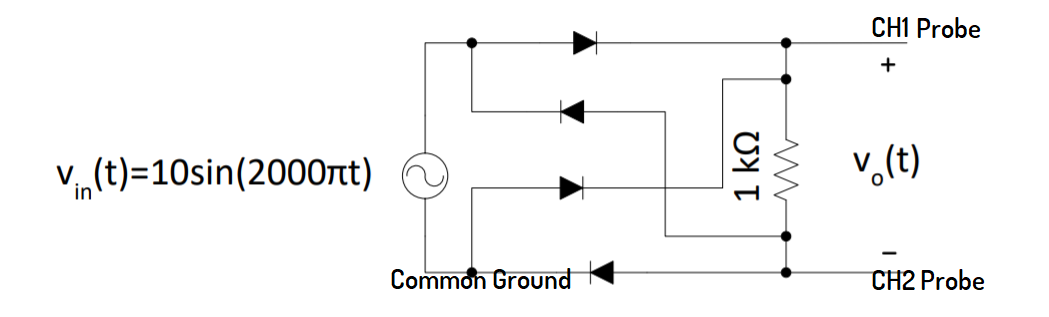
\includegraphics[width=1\textwidth]{full_vave_sch.png}
   \caption{Full wave rectifier circuit}
\end{figure}

\subsubsection{a)}
\begin{figure}[H]
	\centering
   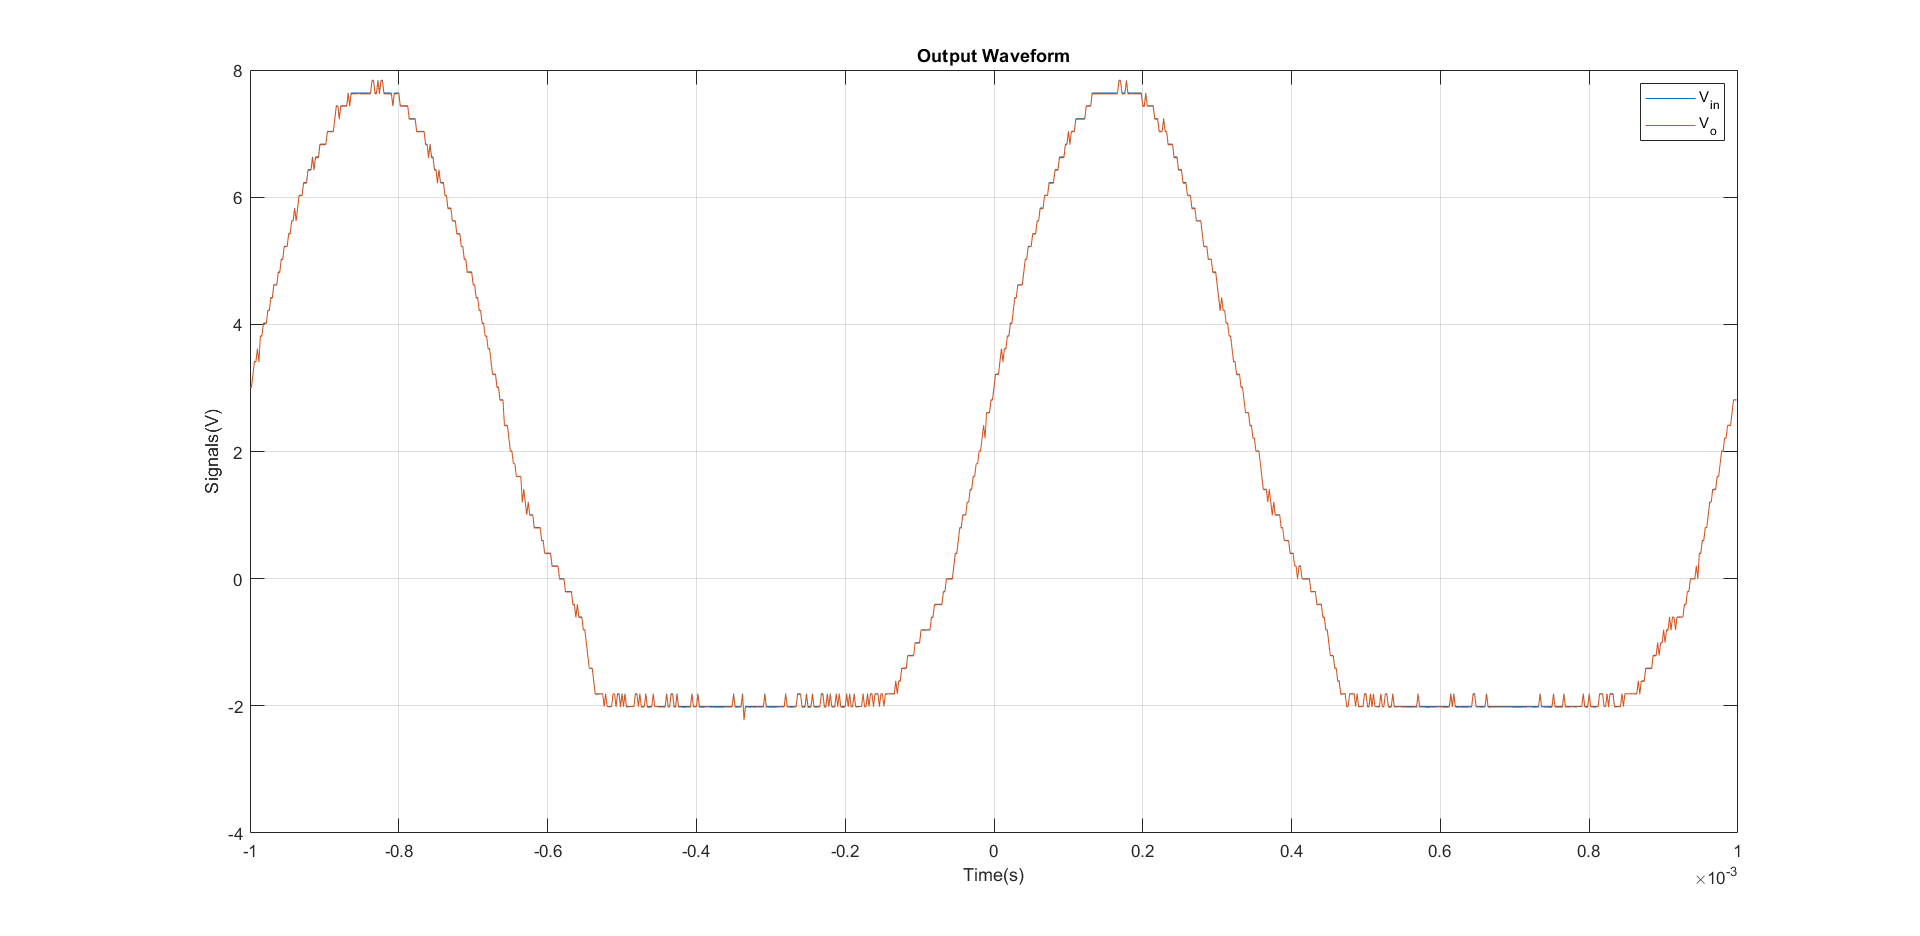
\includegraphics[width=1\textwidth]{2a_plot.png}
   \caption{Output waveforms}
\end{figure}

\subsubsection{b)}

\subsubsection{c)}
\subsection{Step 3}
\begin{figure}[H]
	\centering
   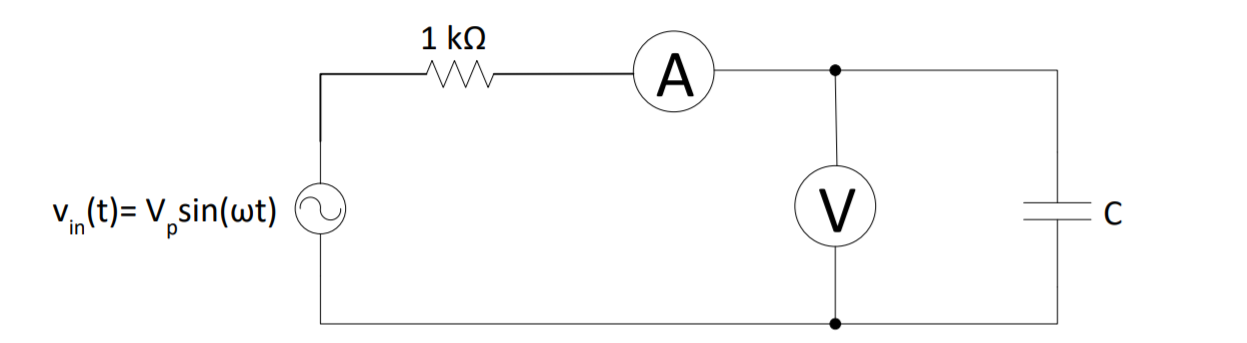
\includegraphics[width=1\textwidth]{PRE3.png}
   \caption{Capacitor measurement circuit}
\end{figure}


\begin{table}[H]
	\begin{center}
		\caption{Measurements for the capacitor circuit}
		\vspace{2mm}
		\begin{tabular}{||c | c | c||} 
		 \hline
		   & Capacitor & Resistor \\ [0.5ex] 
		 \hline\hline
		 Voltage Reading & 1.1518 V & 1.69 V  \\ 
		 \hline
		\end{tabular}
\end{center}
\end{table}
\subsection{Step 4}
\begin{figure}[H]
	\centering
   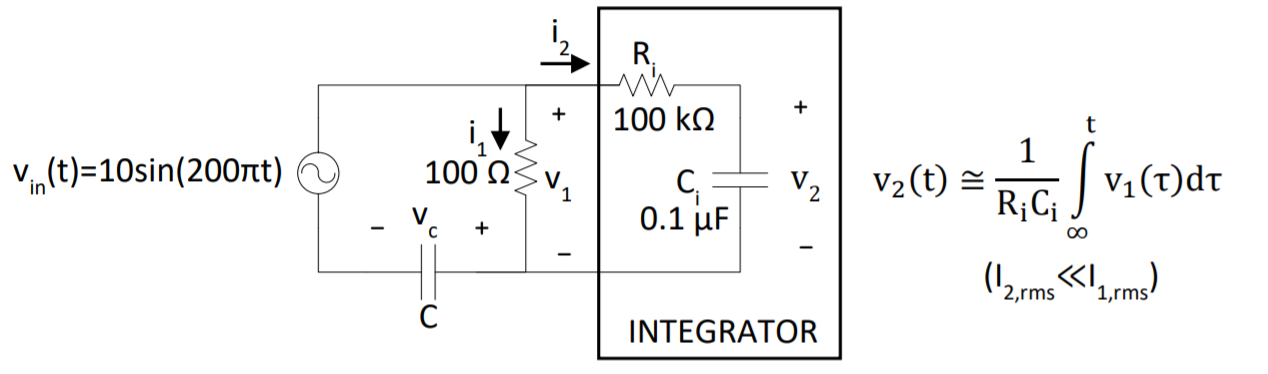
\includegraphics[width=1\textwidth]{PRE4.png}
   \caption{Circuit for the capacitance finding method}
\end{figure}
\begin{figure}[H]
	\centering
   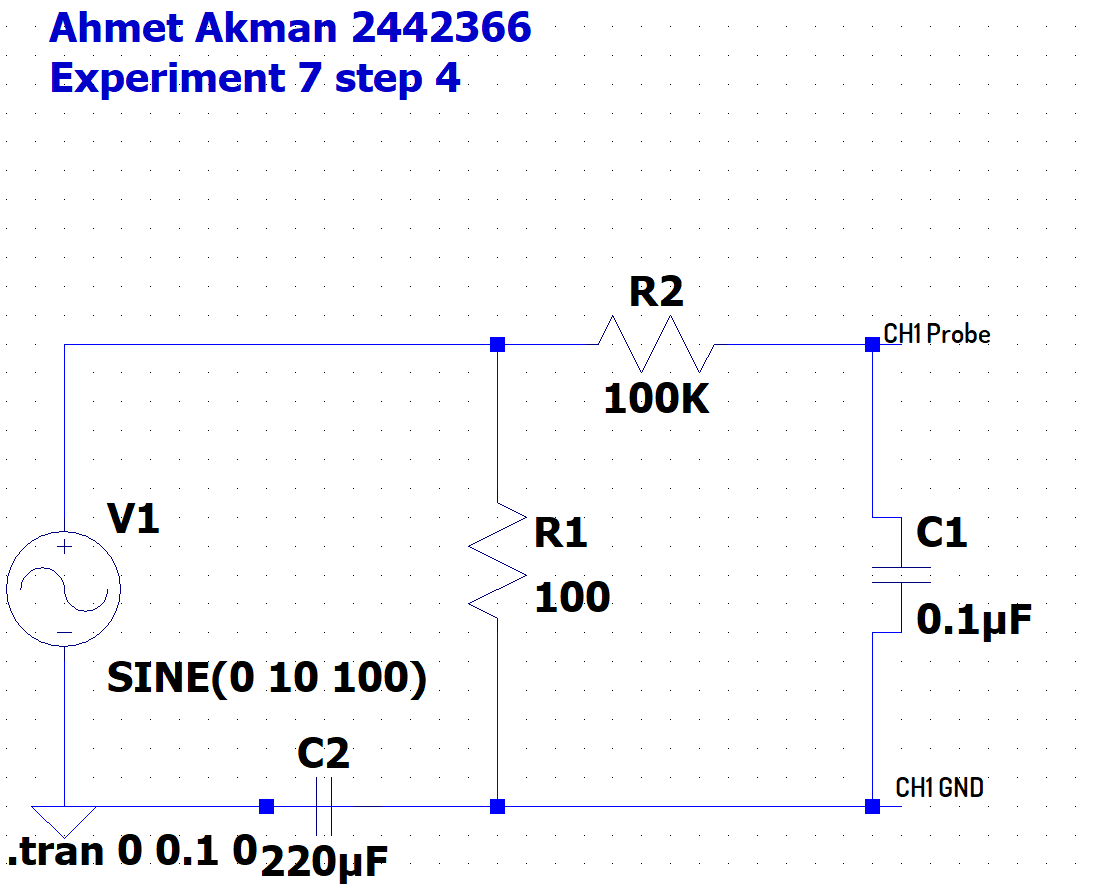
\includegraphics[width=1\textwidth]{4_SCH.png}
   \caption{Simulation circuit for the capacitance finding method}
\end{figure}
\begin{figure}[H]
	\centering
   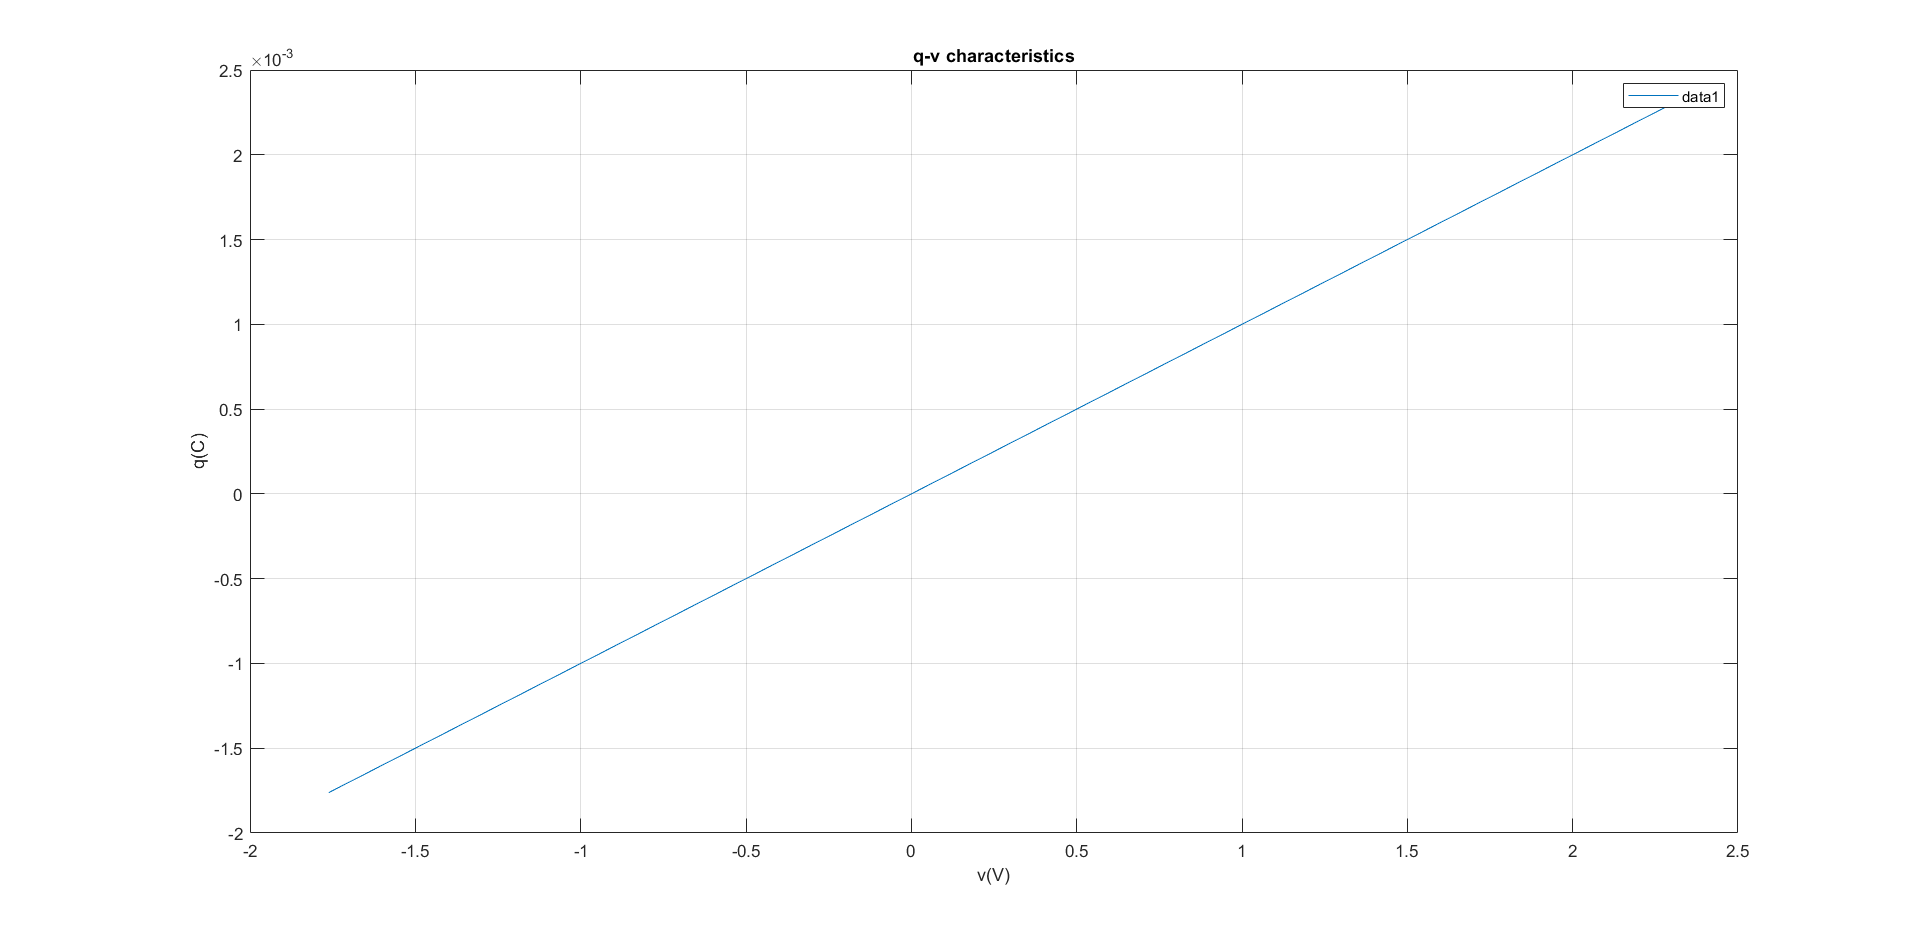
\includegraphics[width=1\textwidth]{4a_plot.png}
   \caption{q-v characteristics}
\end{figure}
%%%% MATHEMATICAL RELATION
\subsection{Step 5}

\begin{table}[H]
	\begin{center}
		\caption{Measurements for the wooden inductor circuit}
		\vspace{2mm}
		\begin{tabular}{||c | c | c||} 
		 \hline
		   & Inductor & Resistor \\ [0.5ex] 
		 \hline\hline
		 Voltage Reading & 0.68321 V & 1.862 V \\
		 \hline
		\end{tabular}
\end{center}
\end{table}

\begin{table}[H]
	\begin{center}
		\caption{Measurements for the compact inductor circuit}
		\vspace{2mm}
		\begin{tabular}{||c | c | c||} 
		 \hline
		   & Inductor & Resistor \\ [0.5ex] 
		 \hline\hline
		 Voltage Reading & 0.59929 V & 1.912 V \\
		 \hline

		\end{tabular}
\end{center}
\end{table}


\begin{table}[H]
	\begin{center}
		\caption{Measurements for the inductors}
		\vspace{2mm}
		\begin{tabular}{||c | c | c||} 
		 \hline
		   & Wooden & Compact \\ [0.5ex] 
		 \hline\hline
		LC Meter Reading & 0.15 H & 0.08 H \\
		 \hline
		Resistance Reading & 29.13 \(\Omega\) & 3.950 \(\Omega\) \\
		 \hline
		\end{tabular}
\end{center}
\end{table}
%%MATHEMATİCAL EXPRESSİON

\subsection{Step 6}
\begin{figure}[H]
	\centering
   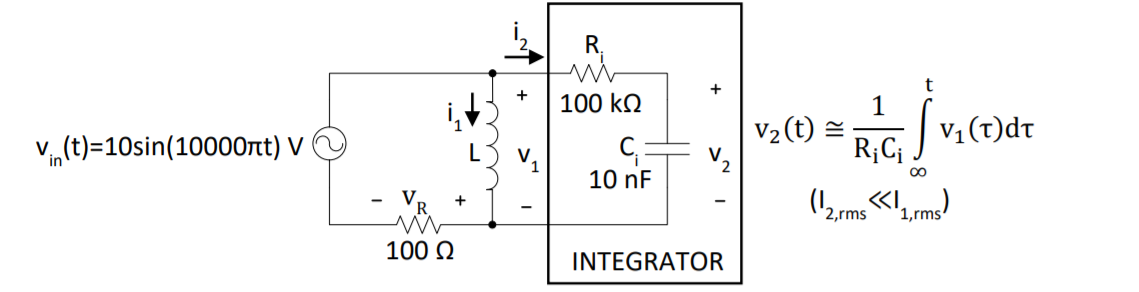
\includegraphics[width=1\textwidth]{PRE7.png}
   \caption{Circuit for the inductance finding method}
\end{figure}

\subsubsection{a)}
\begin{figure}[H]
	\centering
   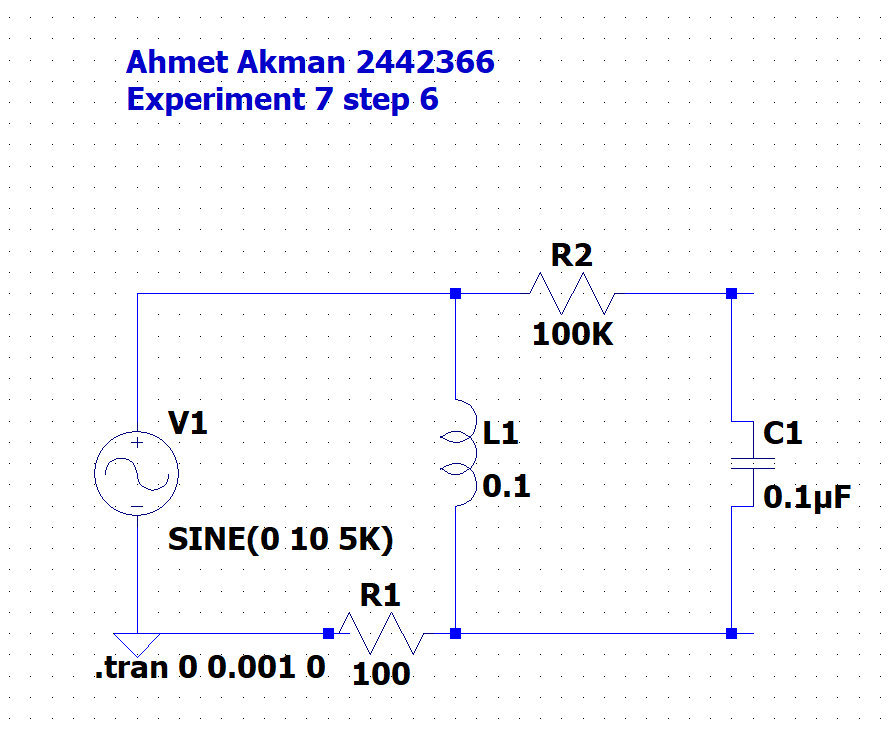
\includegraphics[width=1\textwidth]{6_SCH.png}
   \caption{Simulation circuit for the inductance finding method}
\end{figure}

\begin{figure}[H]
	\centering
   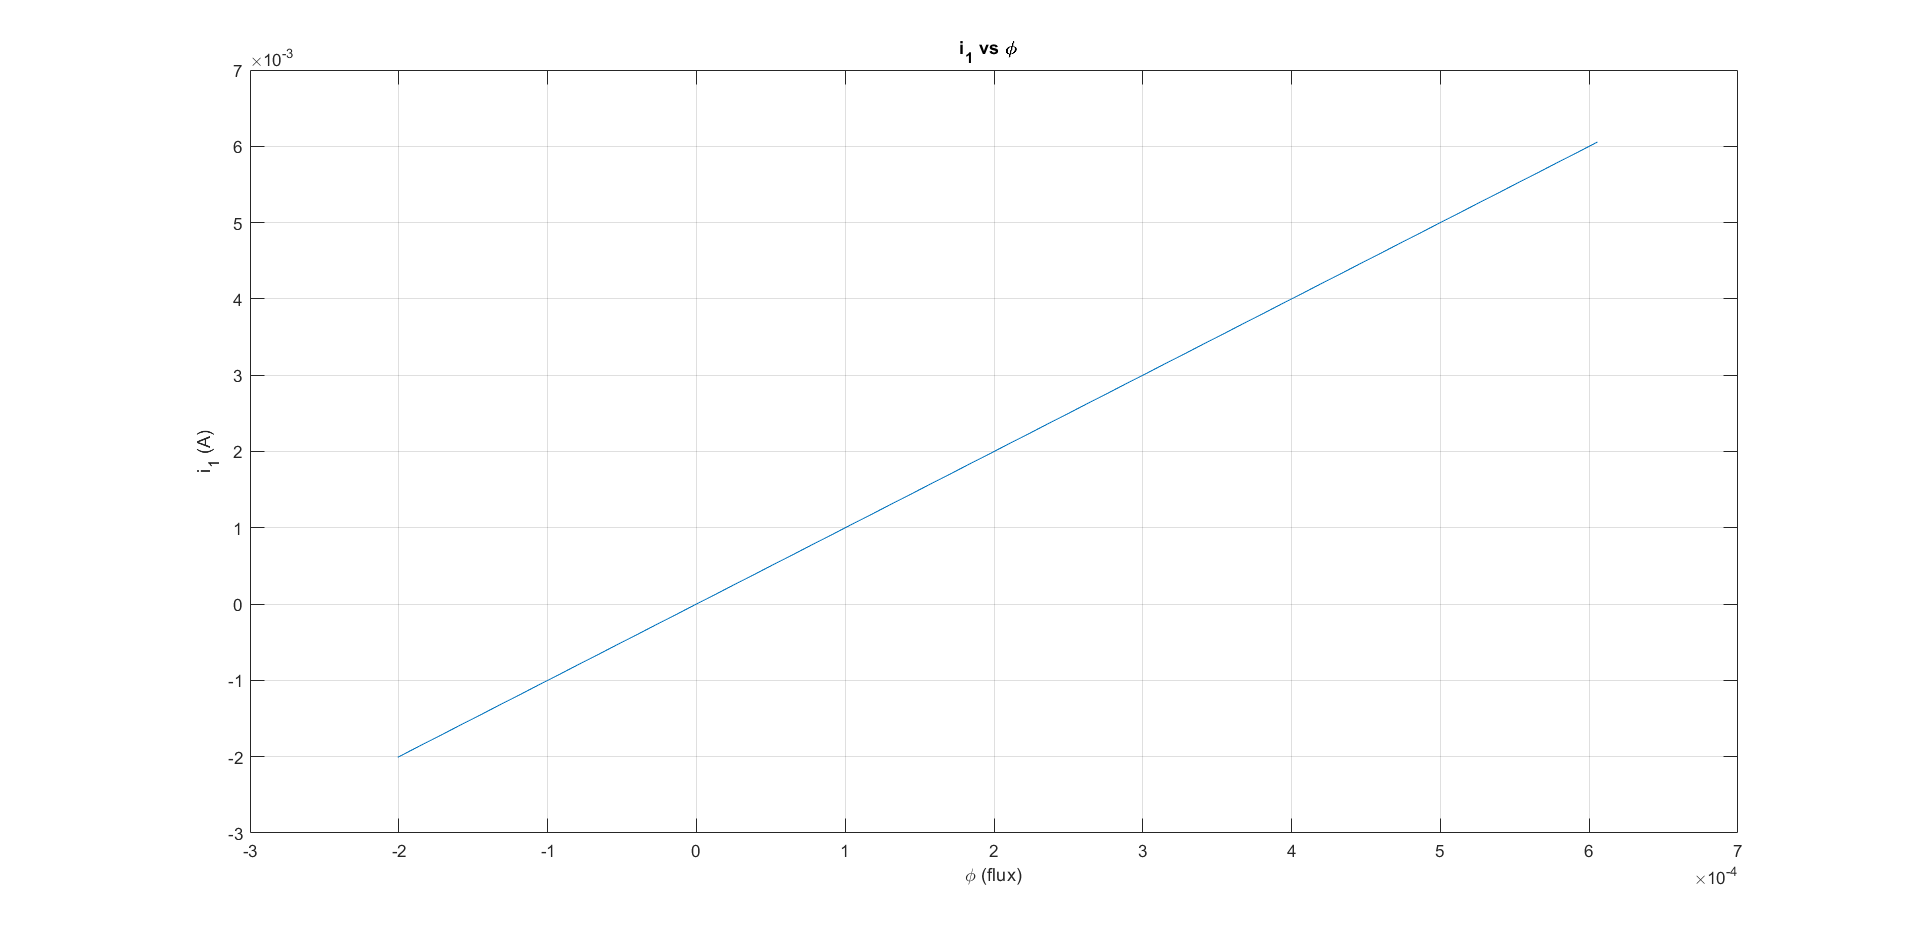
\includegraphics[width=1\textwidth]{PRE_7c.png}
   \caption{\(\phi vs i\) characteristics plot}
\end{figure}
\subsubsection{b)}

\section{Conclusion}
The non-ideal behavior of the components is compared with the ideal simulation plots.

In conclusion, in experiment 6, "Operational Amplifiers-II," as students, we have learned how various functional circuit setups of Op-Amps can be constructed. Preliminary laboratory work is done via simulations of the Op-Amp circuits in an LTSpice environment and by hand calculations. As students, we have observed how the amplifying job can be done in two-stage and its advantages. We have seen the effect of non-linear feedback on the Op-Amp setup. The characteristics of the negative resistance converter are observed. Also, implementing darkness and lightness sensors has experienced a real-life design approach. Lastly, a difference amplifier circuit is set, and the characteristics are observed with measurements. To sum up, in this experiment, as students, we have experimented with how different kinds of operational amplifier circuits operate. 
\section*{Appendix I}
Total time spent on/during:
\begin{itemize}
	\item Pre-lab preparation: 6.5 hours (including the preliminary work and simulations) 
	\item Experimental work: 2 hours (hours spent in lab)
	\item Report writing: 6 hours 
\end{itemize}
\section*{Appendix II}
The outputs of the simulations are fetched from LTSpice and plotted in MATLAB.
%++++++++++++++++++++++++++++++++++++++++
% References section will be created automatically 
% with inclusion of "thebibliography" environment
% as it shown below. See text starting with line
% \begin{thebibliography}{99}
% Note: with this approach it is YOUR responsibility to put them in order
% of appearance.

%\begin{thebibliography}{99}

%https://tr.overleaf.com/latex/templates/sample-lab-report-for-u-of-r-phys-349/pgsyqngcyjxk

%\end{thebibliography}


\end{document}


\begin{table}[H]
	\begin{center}
		\caption{Resistance reading by color code convention.}
		\vspace{2mm}
		\begin{tabular}{||c | c | c||} 
		 \hline
		 Color Order & Value & Tolerance \\ [0.5ex] 
		 \hline\hline
		 Brown / Black / Red / Gold & 1k\( \Omega \) & \( \% \) 5  \\ 
		 \hline
		 Yellow / Violet / Red / Gold & 4.7k\( \Omega \) & \( \% \) 5   \\
		 \hline
		 Brown / Grey / Orange / Gold & 18k\( \Omega \) & \( \% \) 5  \\ [1ex] 
		 \hline
		\end{tabular}
	\end{center}
	\end{table}

	\begin{figure}[H]
 		\centering
		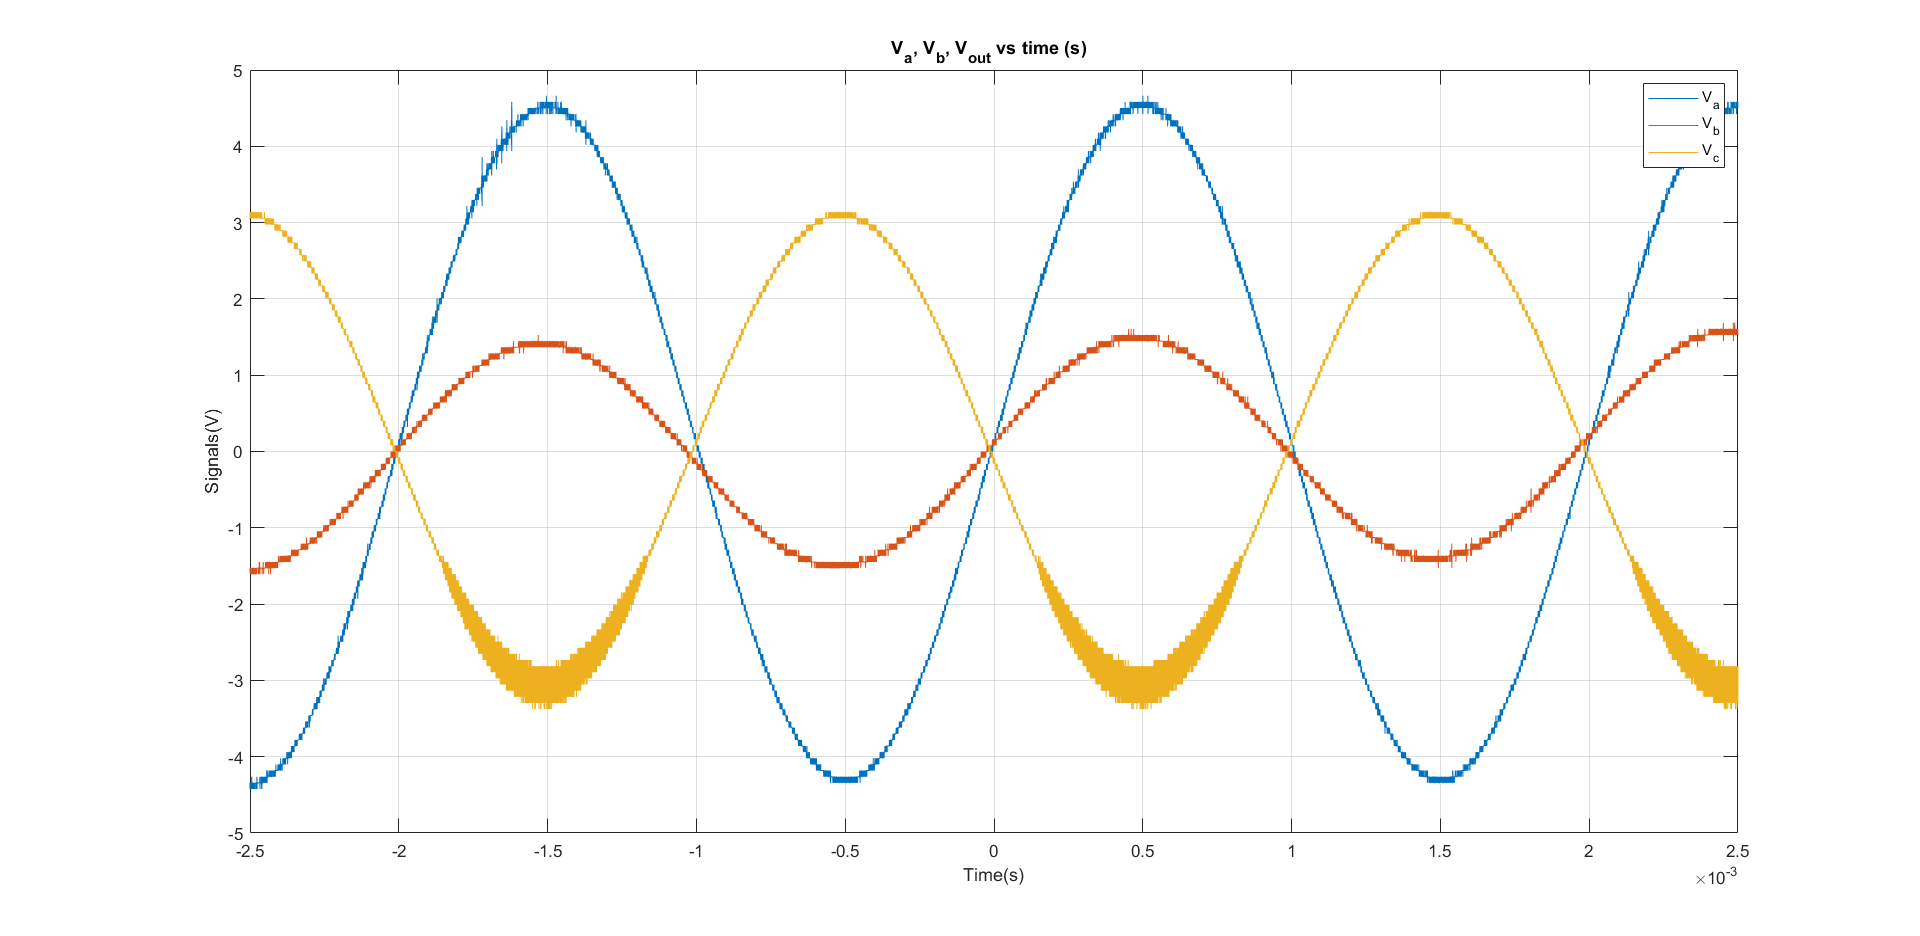
\includegraphics[width=0.6\textwidth]{5.png}
		\caption{Circuit schematic for the step 5}
	\end{figure} 

	\begin{figure}[htp] \centering{
		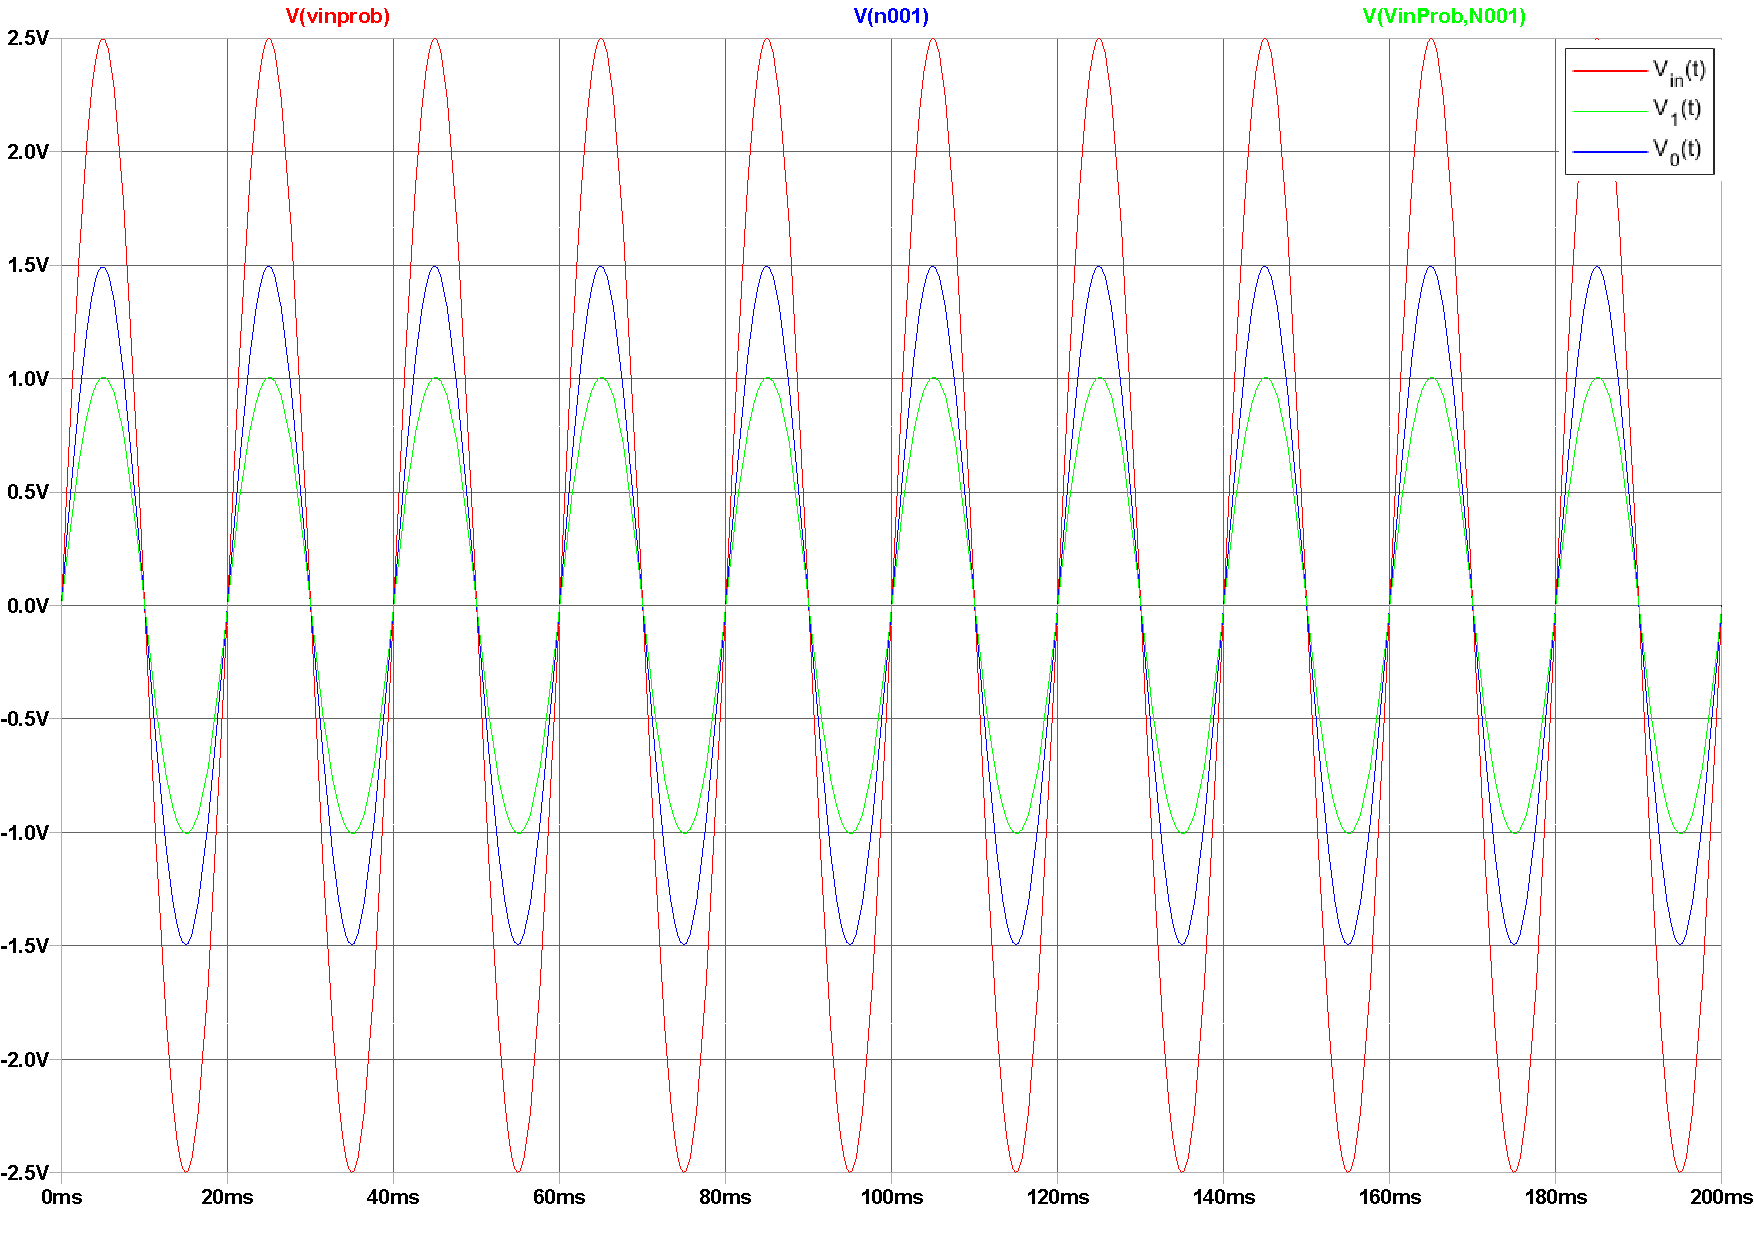
\includegraphics[scale=0.25]{2a_plot.pdf}}
		\caption{Experiment 2}
\end{figure}
	